\documentclass[conference]{IEEEtran}
\IEEEoverridecommandlockouts


% ==================== Packages ====================
\usepackage{cite}
\usepackage{amsmath,amssymb,amsfonts}
\usepackage{graphicx}
\usepackage{textcomp}
\usepackage{xcolor}
\usepackage{booktabs}
\usepackage{multirow}
\usepackage{float}
\usepackage{hyperref}
\usepackage{subcaption}
\usepackage{CJKutf8}
\usepackage{microtype}
\usepackage[english]{babel}

% ==================== 调整正文设置 ====================
% 1. 调整行距：1.3倍行距会让中文看起来更疏朗，视觉上字会显大
\linespread{1.3} 

% ==================== BibTeX Logo ====================
\def\BibTeX{{\rm B\kern-.05em{\sc i\kern-.025em b}\kern-.08em
    T\kern-.1667em\lower.7ex\hbox{E}\kern-.125emX}}

% ==================== Document ====================
\begin{document}
\begin{CJK}{UTF8}{gbsn}

% --- 重命名摘要和关键词为中文 ---
\renewcommand{\abstractname}{摘要}
\renewcommand{\IEEEkeywordsname}{关键词}

% ==================== Title ====================
\title{LFA-Net 复现与视网膜血管分割几何感知增强方法探索}

% ==================== Author ====================
\author{
    \IEEEauthorblockN{\Large 王子腾，杜伟悦，梁欣宇，徐凯威}
    \IEEEauthorblockA{
        BY2506120, ZY2506205, SY2506114, ZY2506427
    }
}

\maketitle


\begin{abstract}
\normalsize
视网膜血管分割对于糖尿病视网膜病变、青光眼等眼科疾病的早期诊断具有重要意义。本文介绍了我们对LFA-Net的复现工作，以及改进其性能的探索性尝试。我们在DRIVE、CHASE\_DB、STARE数据集上复现了LFA-Net基准模型，取得了与原论文相当的结果。随后，我们探索了两种增强策略：（1）显式视盘先验信息融合，（2）几何感知损失函数优化。虽然这些尝试未能提升定量指标，但我们的分析揭示了将先验知识融入轻量级网络的挑战，以及损失函数设计中的权衡问题。本报告详细记录了我们的方法论、实验结果以及从探索过程中获得的经验。
\end{abstract}

\begin{IEEEkeywords}
\normalsize
视网膜血管分割, LFA-Net, 深度学习, 注意力机制, 视盘检测
\end{IEEEkeywords}

\section{引言}

视网膜血管是诊断多种全身性疾病的重要生物标志物。血管形态的变化，如迂曲度、分支模式和管径等，可以指示糖尿病视网膜病变、高血压和心血管疾病等病症\cite{staal2004ridge}。自动化血管分割已成为医学图像分析领域的研究热点。

视网膜血管分割面临的主要挑战包括：
\begin{itemize}
    \item \textbf{类别不平衡}：血管像素通常仅占图像总面积的不到10\%
    \item \textbf{微血管断裂}：细小血管容易出现不连续
    \item \textbf{视盘干扰}：明亮的视盘区域容易产生假阳性
    \item \textbf{血管粗细差异}：粗细血管需要不同的感受野
\end{itemize}

近年来，深度学习方法在医学图像分割领域取得了显著进展。U-Net\cite{ronneberger2015u}建立了编码器-解码器范式，成为医学图像分割的基准模型。后续工作引入了注意力机制\cite{oktay2018attention}、密集连接\cite{li2018h}和多尺度特征融合\cite{chen2017deeplab}等技术进一步提升性能。

在本项目中，我们重点研究LFA-Net\cite{lfanet2025}，这是一个仅有0.11M参数的轻量级网络，通过LiteFusion注意力和Vision Mamba启发的架构实现了优异的性能。我们的工作包括：
\begin{enumerate}
    \item 在DRIVE、CHASE\_DB和STARE数据集上复现LFA-Net
    \item 探索视盘先验信息融合方法
    \item 研究几何感知损失函数
    \item 分析改进方法未能提升性能的原因
\end{enumerate}

\section{相关工作}

\subsection{深度学习血管分割方法}

U-Net\cite{ronneberger2015u}通过跳跃连接建立了编码器-解码器架构，成为医学图像分割的里程碑。Attention U-Net\cite{oktay2018attention}在跳跃连接中引入注意力门控，自动学习关注重要特征。CE-Net\cite{gu2019net}提出了密集空洞卷积和残差多核池化模块。SA-UNet\cite{guo2021sa}引入空间注意力机制增强血管与背景的区分。CS-Net\cite{mou2019cs}设计了曲线结构检测模块专门处理管状结构。

\subsection{轻量级网络设计}

在资源受限的临床环境中部署深度学习模型推动了高效架构的研究。MobileNet\cite{howard2017mobilenets}引入深度可分离卷积大幅减少参数量。EfficientNet\cite{tan2019efficientnet}通过复合缩放优化网络宽度、深度和分辨率。ShuffleNet\cite{zhang2018shufflenet}使用通道混洗实现高效的特征交互。对于医学图像分割，轻量级网络需要在精度和计算效率之间取得平衡。

\subsection{拓扑保持损失函数}

标准的像素级损失（BCE、Dice）往往无法保持血管的连通性。clDice\cite{shit2021cldice}引入基于骨架的监督信号用于管状结构分割。基于距离变换的边界损失\cite{kervadec2019boundary}强制执行几何约束。Tversky损失\cite{salehi2017tversky}通过调节$\alpha$和$\beta$参数控制假阳性和假阴性的权重。Focal Loss\cite{lin2017focal}通过聚焦难分类样本解决类别不平衡问题。

\subsection{视盘检测与分割}

视盘是视网膜图像中的重要解剖结构，准确定位视盘有助于后续的血管分析。传统方法基于颜色和亮度特征进行检测\cite{aquino2010detecting}。近年来，基于深度学习的方法取得了更好的效果，如使用全卷积网络\cite{fu2018joint}和Transformer架构\cite{xie2021segformer}进行端到端的视盘分割。

\section{LFA-Net架构详解}

\subsection{整体架构}

LFA-Net采用高效的编码器-解码器架构，专为资源受限场景设计。其主要创新包括：

\begin{itemize}
    \item \textbf{LiteFusion注意力（LFA）}：结合焦点调制与Vision Mamba启发的动态特征混合
    \item \textbf{区域感知注意力（RAA）}：在跳跃连接中增强空间特征
    \item \textbf{多尺度卷积}：并行使用不同核大小和膨胀率的卷积
\end{itemize}

图\ref{fig:architecture}展示了LFA-Net的整体网络架构，包括编码器、解码器、LFA模块和RAA注意力机制的连接方式。

\begin{figure}[htbp]
\centering
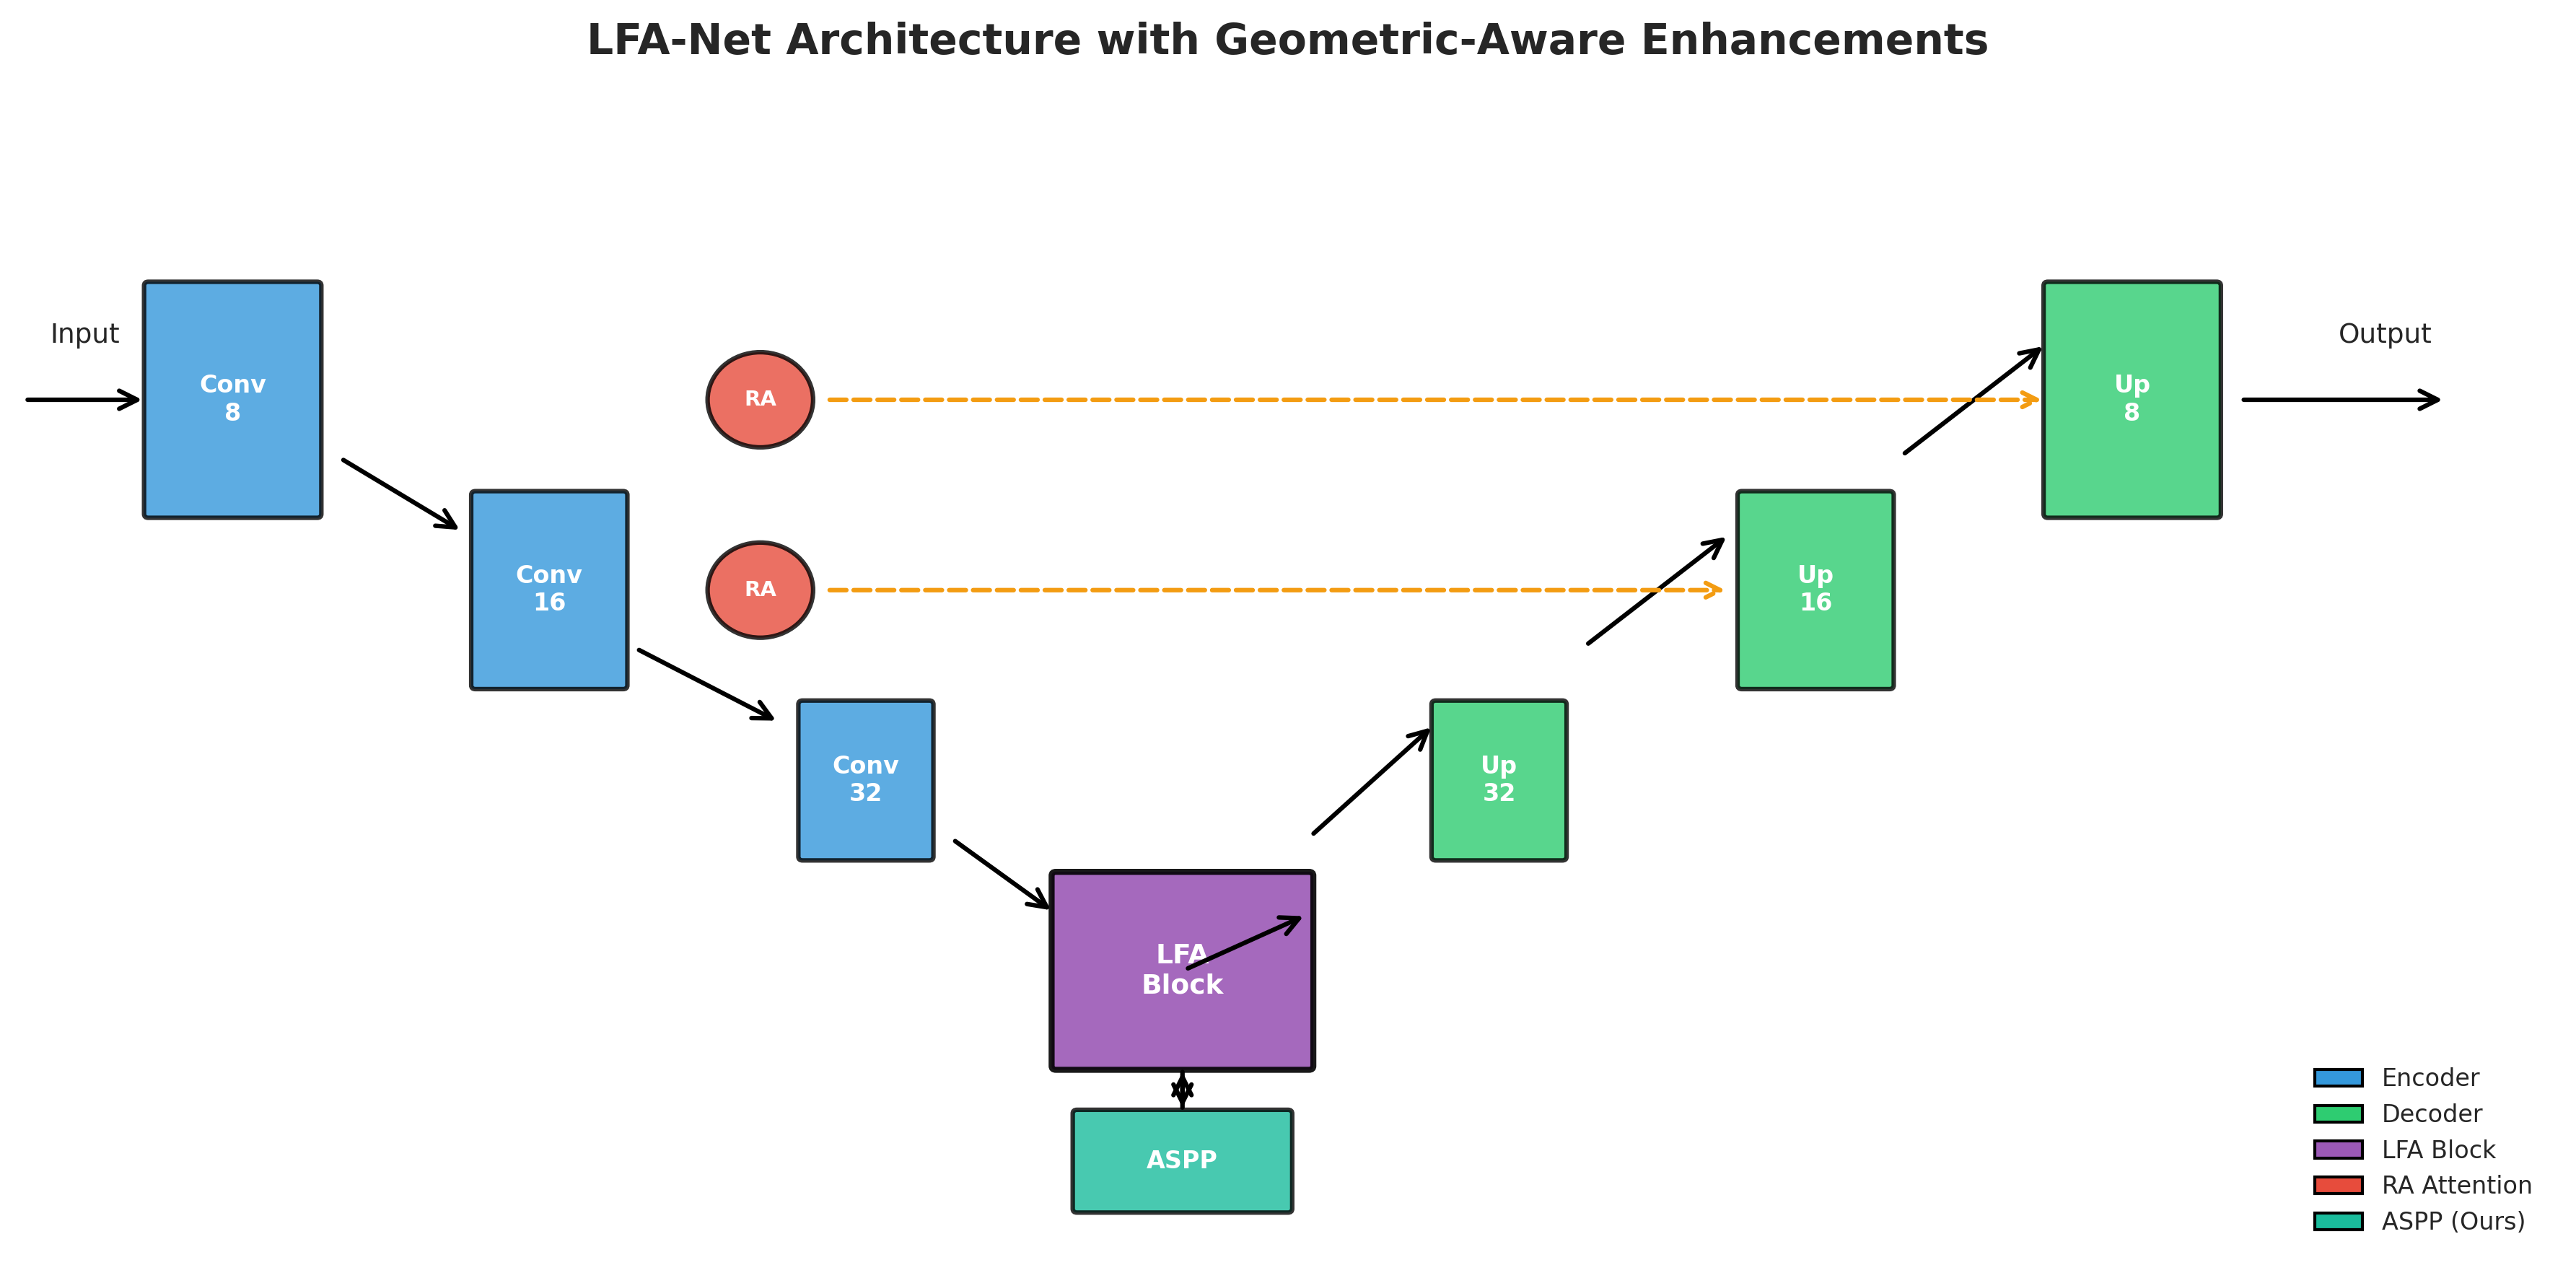
\includegraphics[width=0.95\columnwidth]{figures/architecture.png}
\caption{LFA-Net网络架构示意图。网络采用编码器-解码器结构，在瓶颈层使用LiteFusion Attention (LFA) 模块，在跳跃连接中使用Region-Aware (RA) 注意力机制。图中还展示了我们尝试添加的ASPP模块位置。}
\label{fig:architecture}
\end{figure}

\subsection{LiteFusion注意力模块}

LFA模块是网络瓶颈层的核心组件，包含以下子模块：

\subsubsection{焦点调制（Focal Modulation）}
\begin{equation}
    \text{FM}(x) = x^{\gamma} \cdot \sigma(\text{Conv}(\text{GAP}(x) - \text{GMP}(x)))
\end{equation}
其中$\gamma$是焦点参数，GAP和GMP分别表示全局平均池化和全局最大池化。该模块通过差分池化捕获全局上下文信息。

\subsubsection{焦点调制上下文聚合（FMCA）}
FMCA将局部卷积特征与全局上下文相结合：
\begin{equation}
    \text{FMCA}(x) = \text{Concat}[\text{Conv}_{3\times3}(x), \text{FM}(\text{Conv}_{1\times1}(x))]
\end{equation}

\subsubsection{Vision Mamba启发模块}
该模块通过深度卷积和通道混合提供高效的token交互：
\begin{equation}
    \text{VM}(x) = x + \text{MLP}(\text{LN}(x + \text{DWConv}(\text{LN}(x))))
\end{equation}
其中LN表示层归一化，DWConv表示深度卷积，MLP是多层感知机。

\subsection{区域感知注意力}

RAA用于跳跃连接以增强相关空间特征：
\begin{equation}
    \text{RAA}(x) = x \odot \text{mean}(\text{GAP}(f) \cdot \text{GMP}(f))
\end{equation}
其中$f = \text{Conv}(x)$重塑为$(B, H, W, C, K)$的形状。

\subsection{多尺度ConvBlock}

每个编码器块使用并行卷积捕获多尺度特征：
\begin{equation}
    \text{ConvBlock}(x) = \text{LReLU}(f_{1\times1}(x) + f_{3\times3}(x) + f_{d3\times3}(x))
\end{equation}
其中$f_{d3\times3}$是膨胀率为2的空洞卷积，LReLU是Leaky ReLU激活函数。

\section{基准模型复现}

\subsection{数据集}

我们在三个公开的视网膜血管分割数据集上进行评估：

\begin{itemize}
    \item \textbf{DRIVE}\cite{staal2004ridge}：40张图像（20张训练/20张测试），分辨率$565 \times 584$
    \item \textbf{CHASE\_DB}\cite{fraz2012ensemble}：28张图像（20张训练/8张测试），分辨率$999 \times 960$
    \item \textbf{STARE}\cite{hoover2000locating}：20张图像（16张训练/4张测试），分辨率$700 \times 605$
\end{itemize}

按照原论文的设置，我们采用数据增强策略，包括每20度旋转和对比度调整：
\begin{itemize}
    \item DRIVE：1080张增强后的训练图像
    \item STARE：1024张增强后的训练图像
    \item CHASE\_DB：1080张增强后的训练图像
\end{itemize}

\subsection{实现细节}

\begin{itemize}
    \item 框架：PyTorch
    \item 优化器：Adam（学习率 = $1\times10^{-3}$）
    \item 批大小：64
    \item 训练轮数：200
    \item 损失函数：DiceBCE Loss
    \item 图像尺寸：$560 \times 560$（缩放后）
\end{itemize}

\subsection{基准结果}

表\ref{tab:baseline}展示了我们在三个数据集上复现的基准结果。

\begin{table}[htbp]
\caption{三个数据集上的LFA-Net基准结果}
\label{tab:baseline}
\centering
\setlength{\tabcolsep}{4pt} % 微调列间距以适应更多数据
\begin{tabular}{@{}lcccccc@{}}
\toprule
\textbf{数据集} & \textbf{IoU} & \textbf{F1} & \textbf{敏感度} & \textbf{精确度} & \textbf{准确率} & \textbf{特异度} \\
\midrule
DRIVE     & 0.631 & 0.773 & 0.698 & 0.873 & 0.965 & 0.990 \\
CHASE\_DB & 0.648 & 0.786 & 0.719 & 0.868 & 0.972 & 0.992 \\
STARE     & 0.573 & 0.729 & 0.667 & 0.814 & 0.964 & 0.988 \\
\bottomrule
\end{tabular}
\end{table}

\subsection{训练曲线}

图\ref{fig:loss_curves}展示了三个数据集上的训练和验证损失曲线。模型在大约75-100轮后稳定收敛。

\begin{figure}[htbp]
\centering
\begin{subfigure}[b]{0.32\columnwidth}
    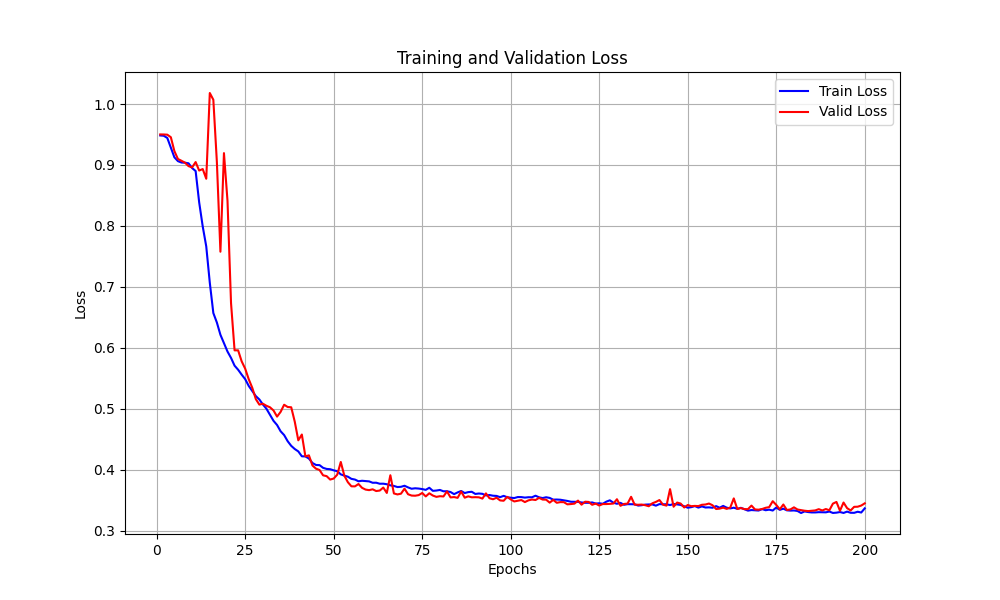
\includegraphics[width=\textwidth]{figures/loss_drive.png}
    \caption{DRIVE}
\end{subfigure}
\begin{subfigure}[b]{0.32\columnwidth}
    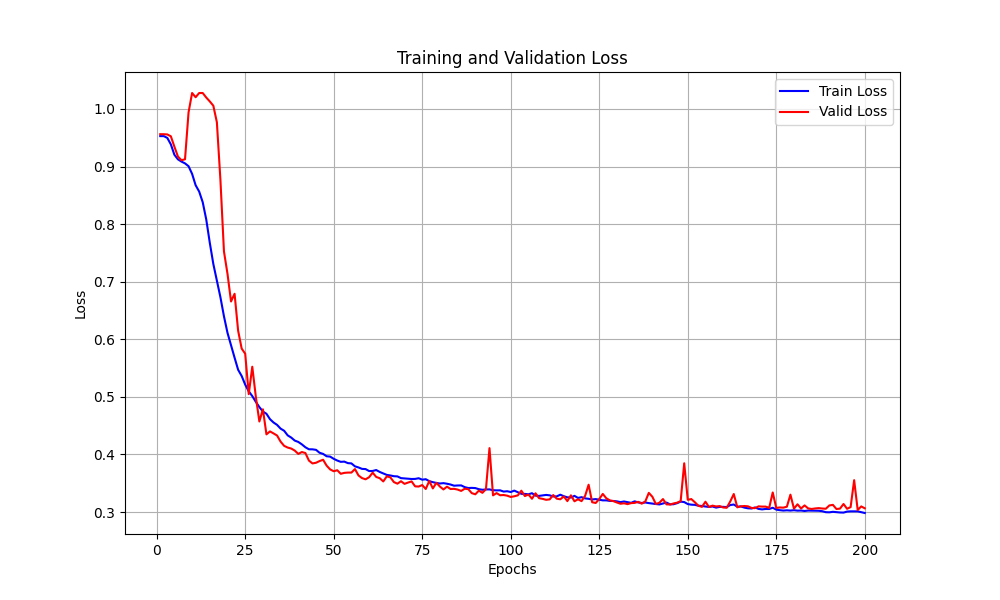
\includegraphics[width=\textwidth]{figures/loss_chase.png}
    \caption{CHASE\_DB}
\end{subfigure}
\begin{subfigure}[b]{0.32\columnwidth}
    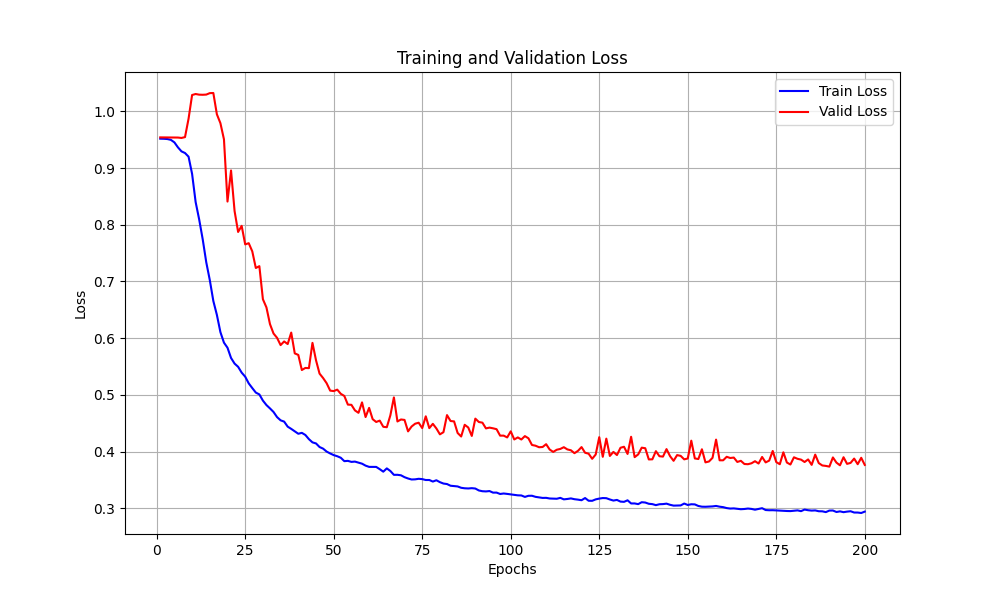
\includegraphics[width=\textwidth]{figures/loss_stare.png}
    \caption{STARE}
\end{subfigure}
\caption{LFA-Net在三个数据集上的训练和验证损失曲线。DRIVE和CHASE\_DB显示出良好的训练-验证对齐，而STARE存在一定的过拟合现象。}
\label{fig:loss_curves}
\end{figure}

基准模型展现了均衡的性能，但存在两个主要问题：
\begin{enumerate}
    \item 视盘边界附近的假阳性较多
    \item 外周微血管存在断裂现象
\end{enumerate}

\section{探索一：视盘先验信息融合}

\subsection{动机}

视盘（Optic Disc, OD）是视网膜图像中的高亮度圆形区域，主要血管在此汇聚。我们假设提供显式的视盘位置信息可以帮助网络：
\begin{itemize}
    \item 抑制视盘边界处的假阳性预测
    \item 更好地区分血管与明亮的视盘背景
\end{itemize}

\subsection{方法}

我们采用多阶段方法：

\subsubsection{视盘掩码生成}
使用预训练的SegFormer模型\cite{xie2021segformer}（经过视盘/视杯分割微调）自动生成视盘掩码。

\subsubsection{视盘区域颜色调和}
应用基于距离的颜色调和处理视盘区域周围，减少视盘边界处的强度不连续性。

\subsubsection{特征工程}
构建3通道特征堆叠：[绿色通道, CLAHE增强, TopHat形态学]以增强血管可见性。

\subsubsection{预处理流程}

图\ref{fig:pipeline_combined}展示了完整的预处理流程，包括视盘融合、特征工程和数据增强。

\begin{figure*}[htbp]
    \centering
    % --- 左侧图片 (样本1) ---
    \begin{subfigure}{0.48\textwidth}
        \centering
        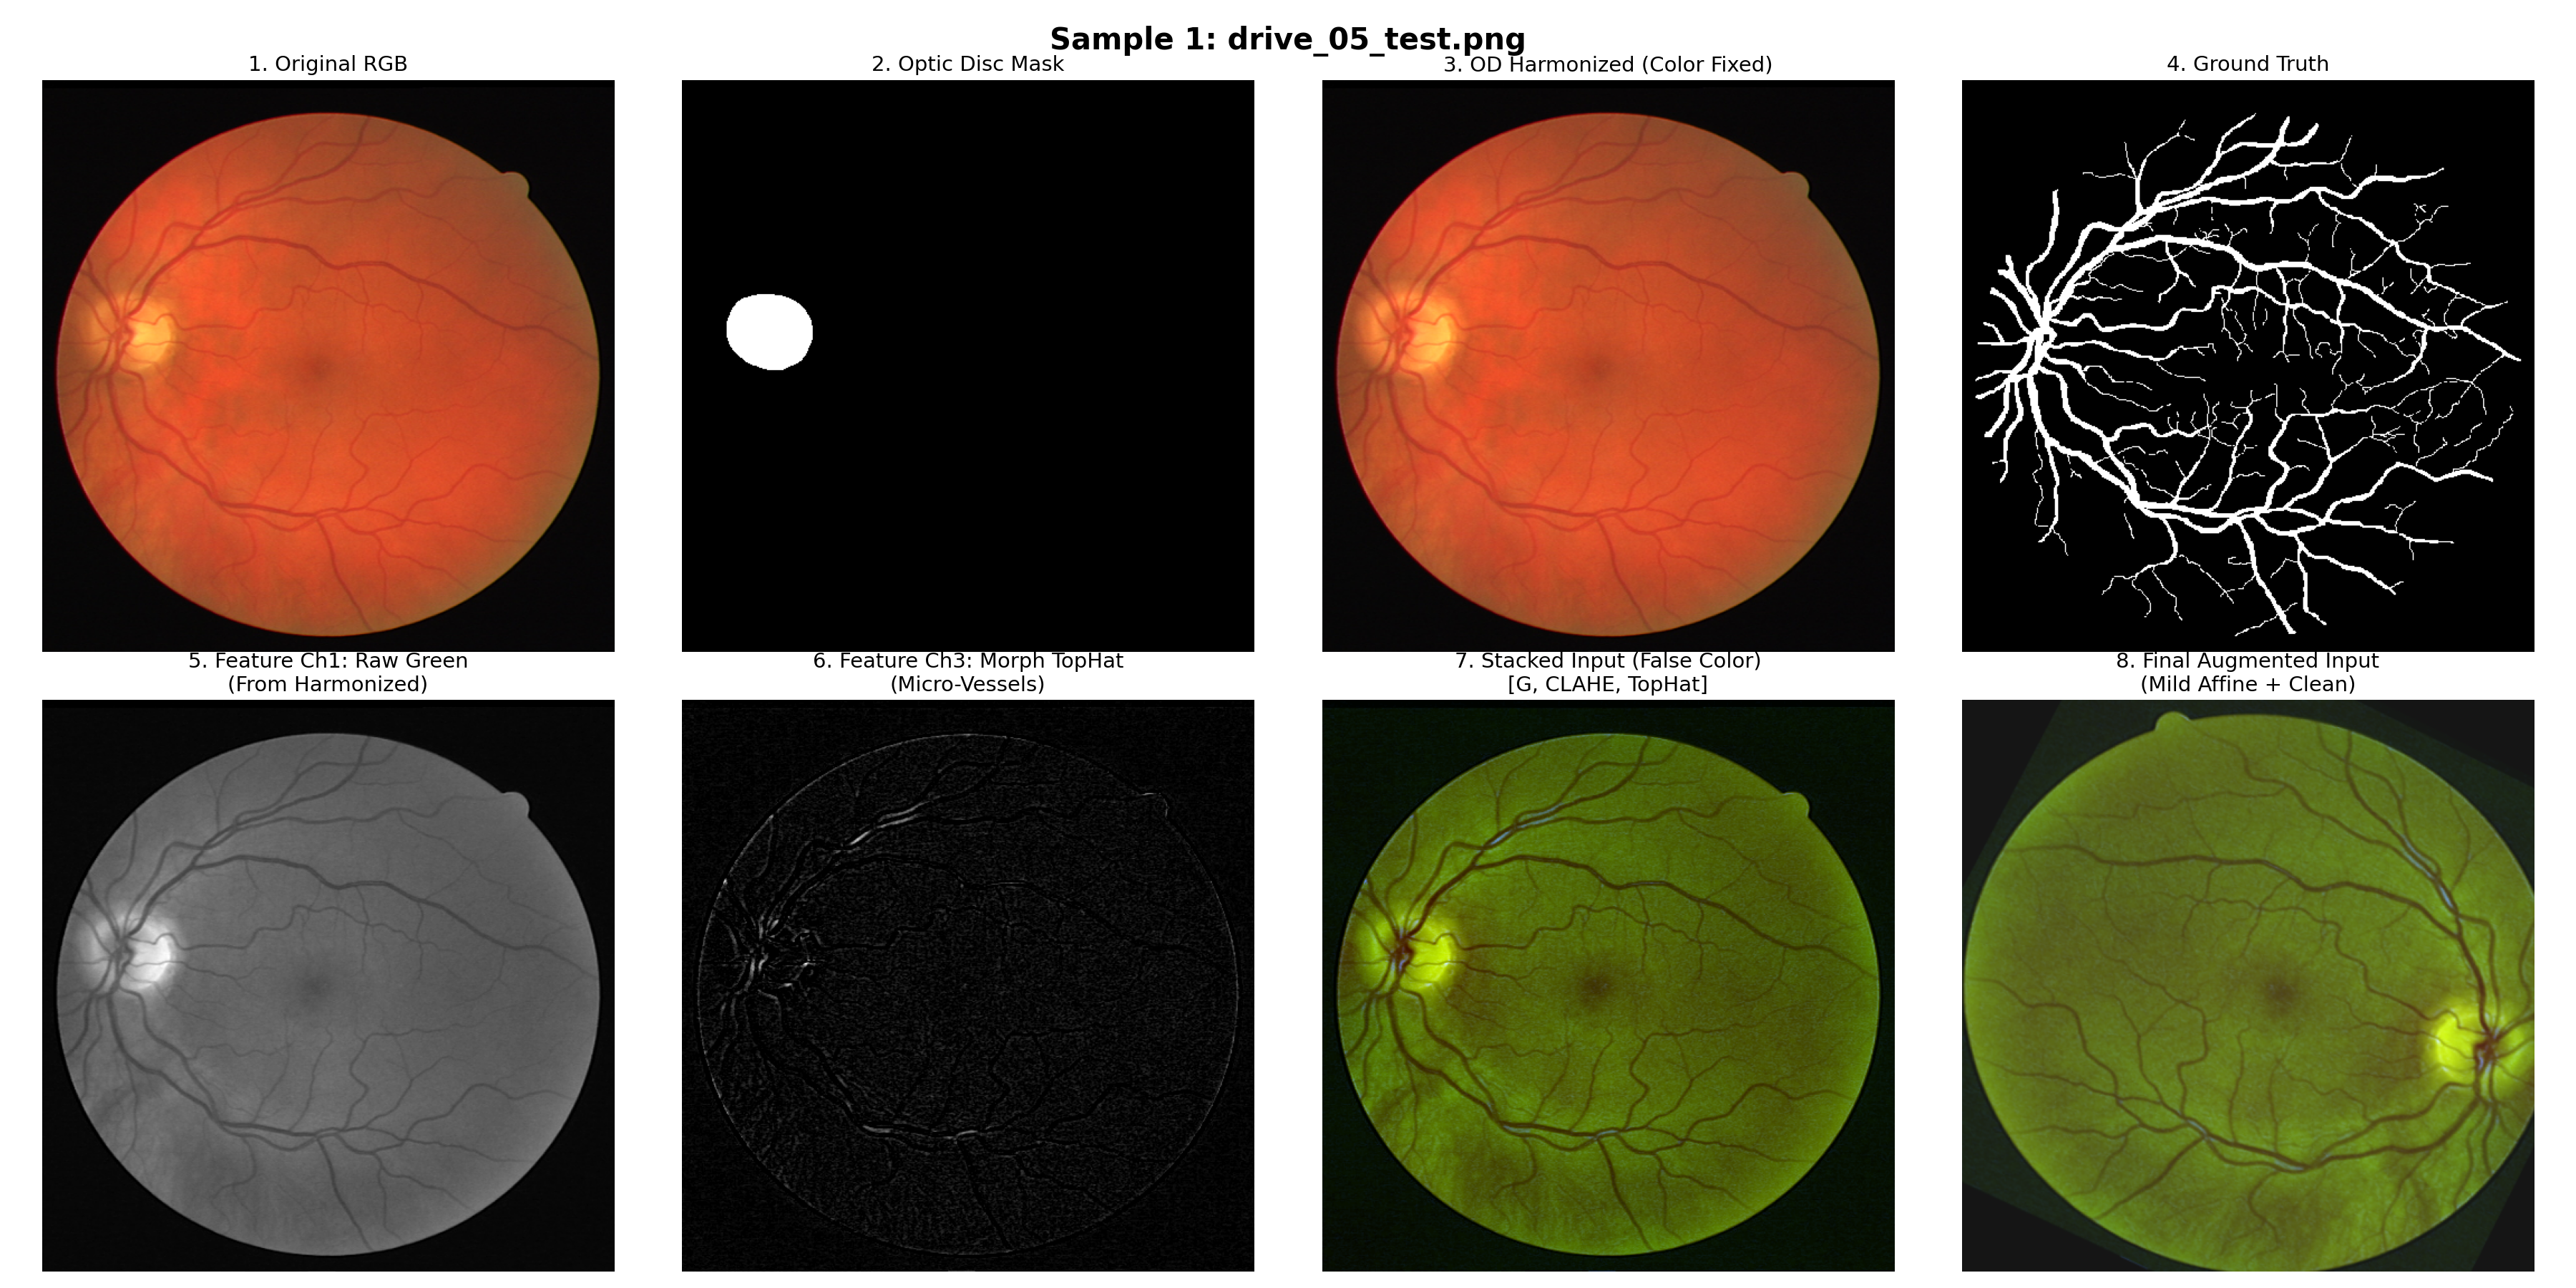
\includegraphics[width=\linewidth]{figures/pipeline_vis_0.png}
        \caption{预处理流程示例（样本1）}
        \label{fig:pipeline_s1}
    \end{subfigure}
    \hfill % 在两图之间通过填充撑开距离
    % --- 右侧图片 (样本2) ---
    \begin{subfigure}{0.48\textwidth}
        \centering
        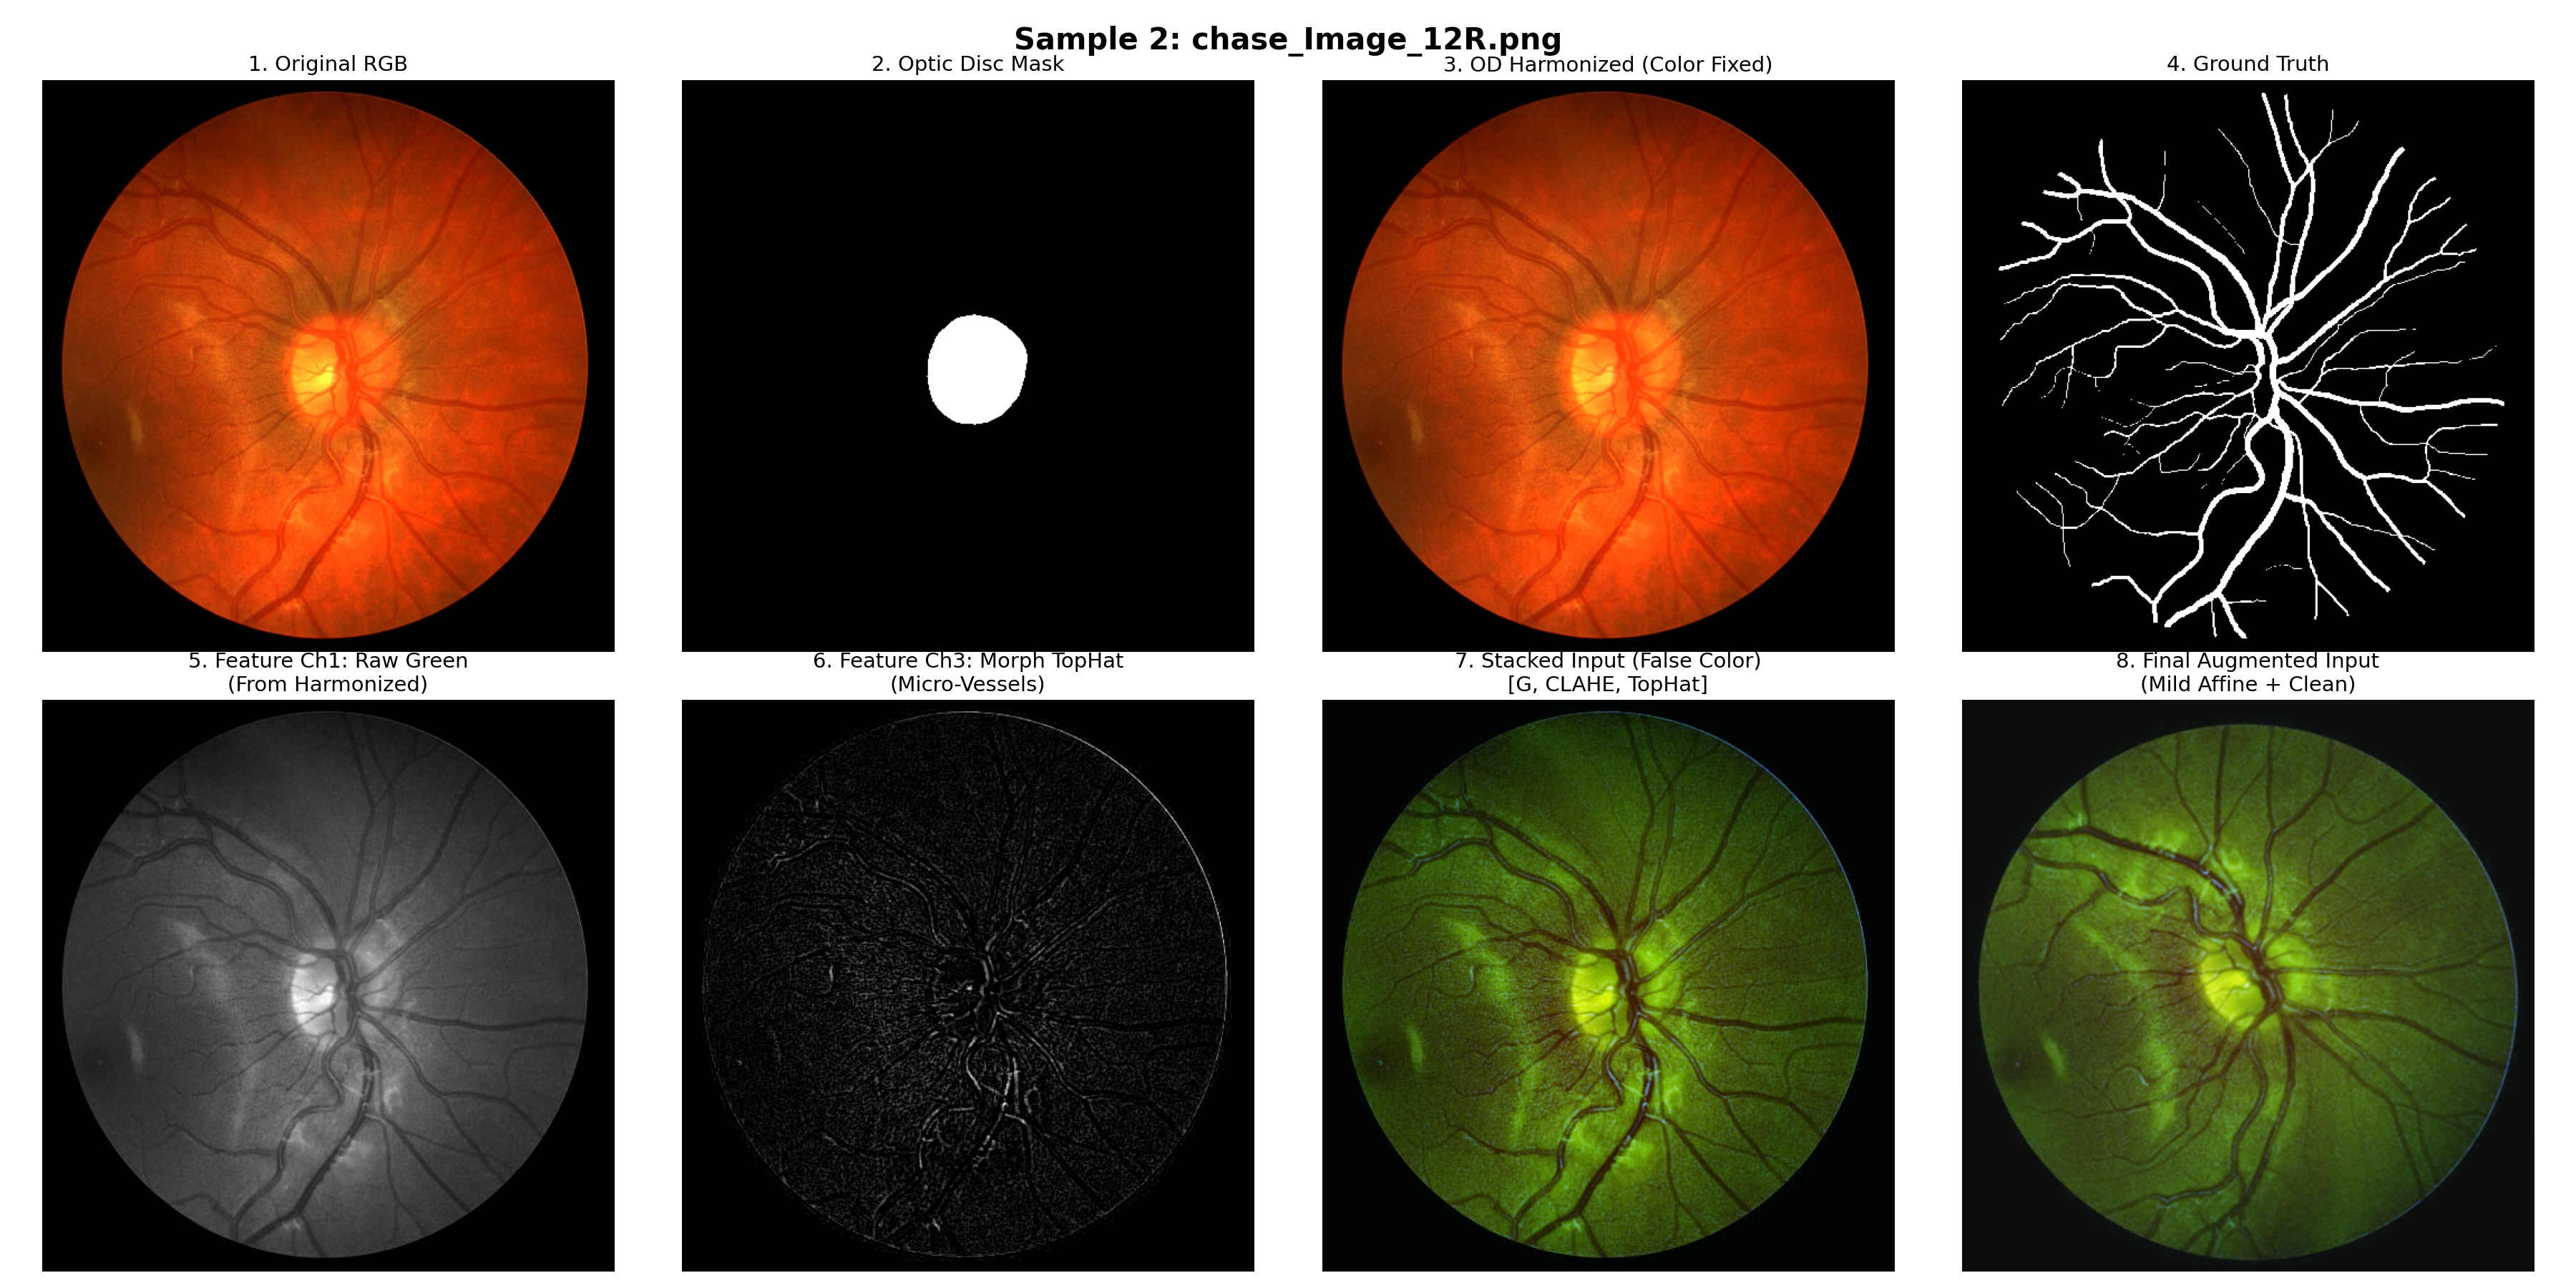
\includegraphics[width=\linewidth]{figures/pipeline_vis_1.png}
        \caption{预处理流程示例（样本2）}
        \label{fig:pipeline_s2}
    \end{subfigure}

    % --- 统一的图注 ---
    \caption{数据预处理流程可视化。图(a)和图(b)展示了不同眼底图像经过相同流程的处理效果。图中每行从左到右依次为：(1)原始RGB图像，(2)自动生成的视盘掩码，(3)视盘区域颜色调和后的图像，(4)血管标注真值，(5)绿色通道提取，(6)形态学TopHat变换用于微血管增强，(7)堆叠特征输入[G, CLAHE, TopHat]，(8)最终增强后的输入图像。}
    \label{fig:pipeline_combined}
\end{figure*}

\subsection{实验结果}

表\ref{tab:od_results}展示了视盘先验融合实验的结果。

\begin{table}[htbp]
\caption{视盘先验融合实验结果}
\label{tab:od_results}
\centering
\begin{tabular}{@{}lccc@{}}
\toprule
\textbf{方法} & \textbf{IoU} & \textbf{F1} & \textbf{变化} \\
\midrule
\multicolumn{4}{c}{\textit{输入通道拼接}} \\
\midrule
基准（DRIVE） & 0.6305 & 0.7728 & -- \\
+ 视盘输入 & 0.6240 & 0.7681 & $\downarrow$ 1.0\% \\
\midrule
\multicolumn{4}{c}{\textit{推理时显式视盘处理}} \\
\midrule
DRIVE（优化）     & 0.6245 & 0.7683 & $\downarrow$ 0.95\% \\
CHASE\_DB（优化） & 0.6340 & 0.7752 & $\downarrow$ 2.21\% \\
STARE（优化）     & 0.5544 & 0.7128 & $\downarrow$ 3.31\% \\
\bottomrule
\end{tabular}
\end{table}

\textbf{关键发现}：所有方法均导致性能下降而非提升。

\subsection{可视化对比}

图\ref{fig:all_od_results}展示了基准模型与视盘优化模型的对比结果。误差图中：绿色=真阳性，红色=假阴性，蓝色=假阳性。

\begin{figure*}[p] % [p] 表示单独成页，防止高度不够
    \centering
    
    % --- 1. DRIVE 01 ---
    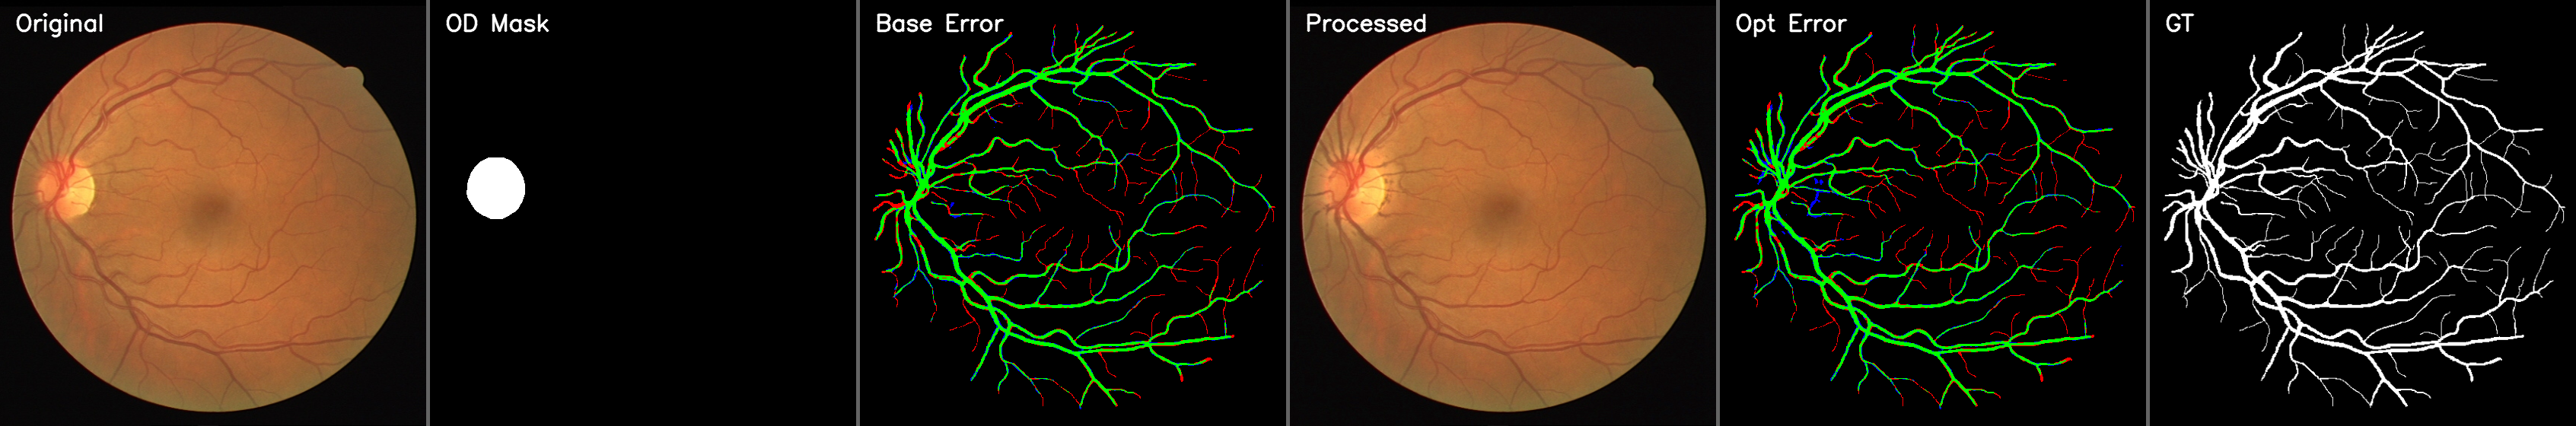
\includegraphics[width=0.9\linewidth]{figures/od_result_drive_01.png}
    \vspace{1pt} % 微调垂直间距
    
    % --- 2. DRIVE 02 ---
    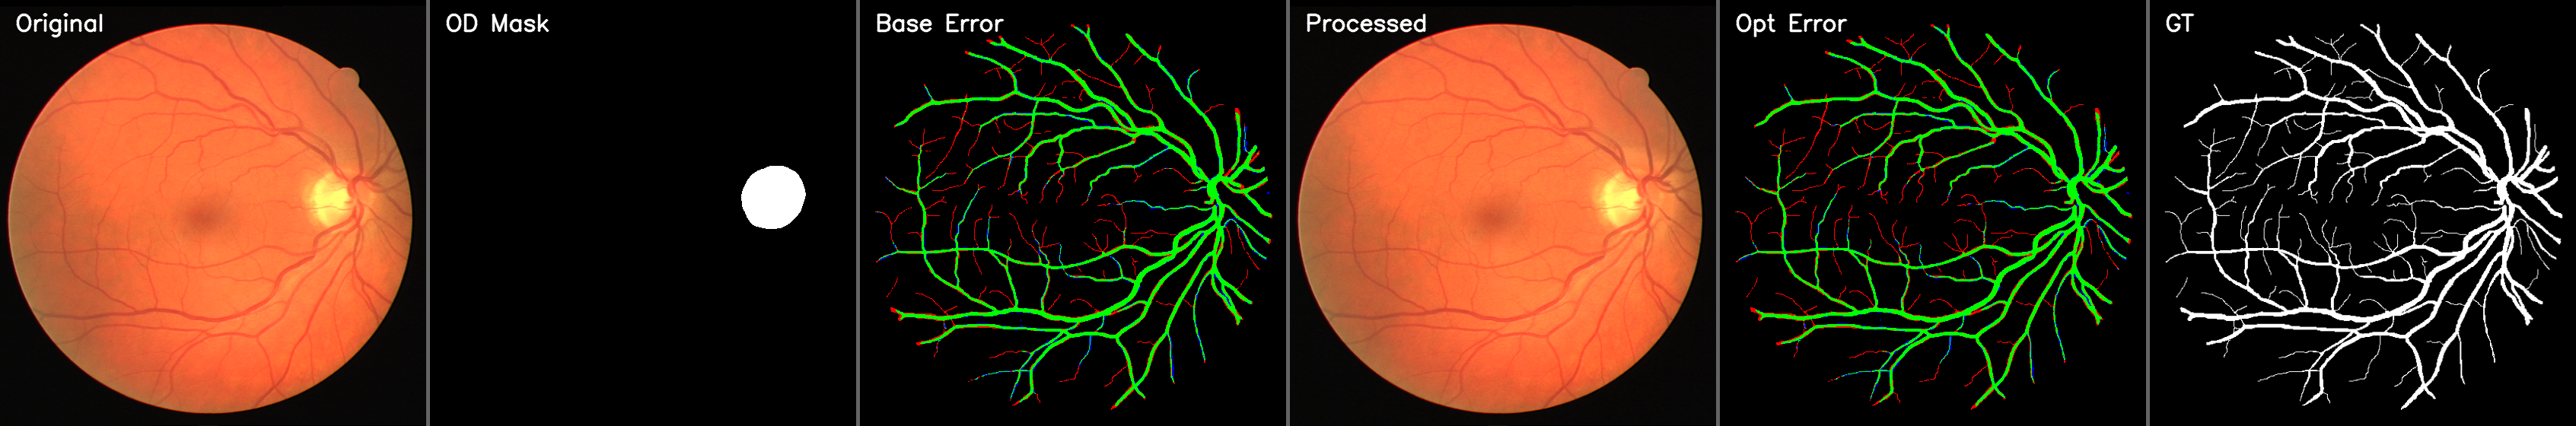
\includegraphics[width=0.9\linewidth]{figures/od_result_drive_02.png}
    \vspace{1pt}
    
    % --- 4. DRIVE 05 ---
    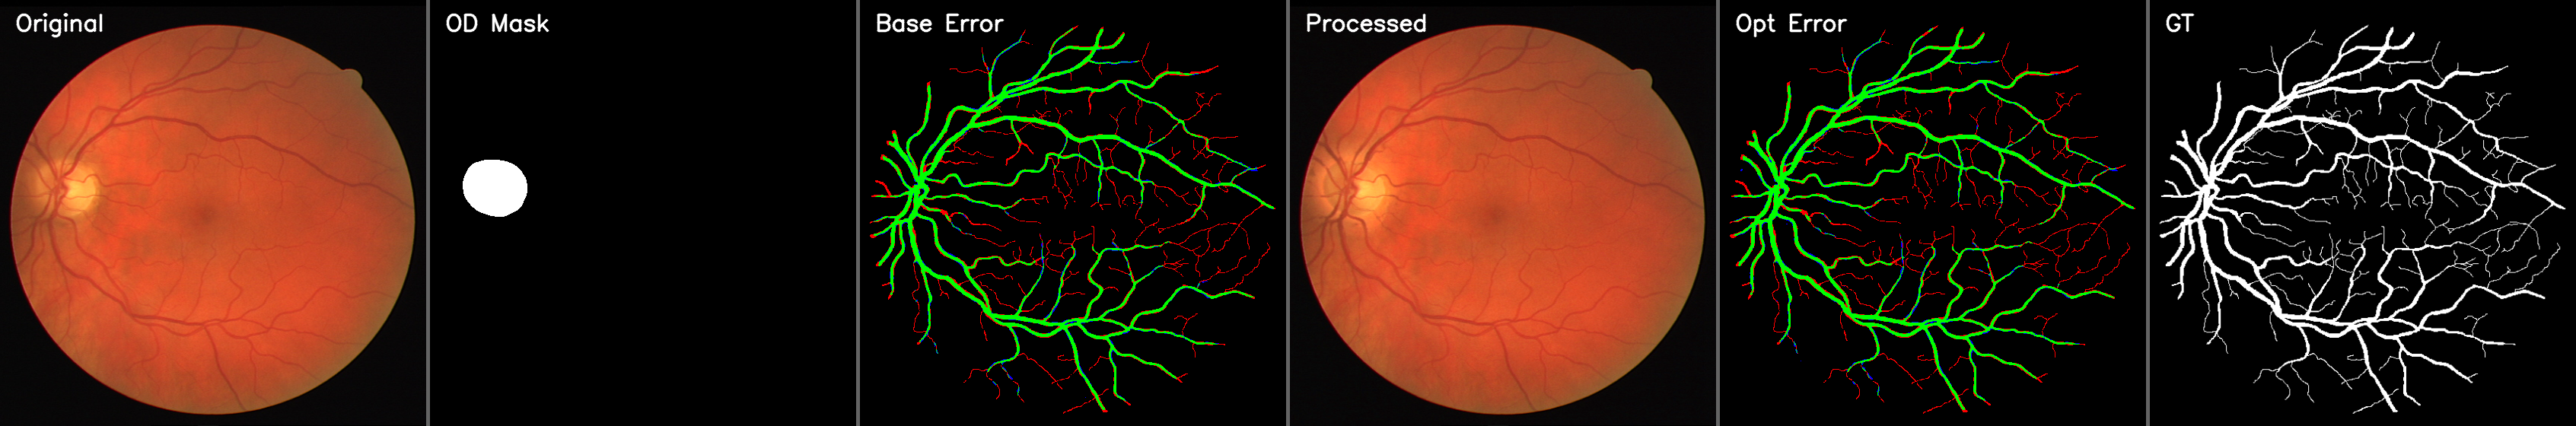
\includegraphics[width=0.9\linewidth]{figures/od_result_drive_05.png}
    \vspace{1pt}
    
    % --- 5. DRIVE 10 ---
    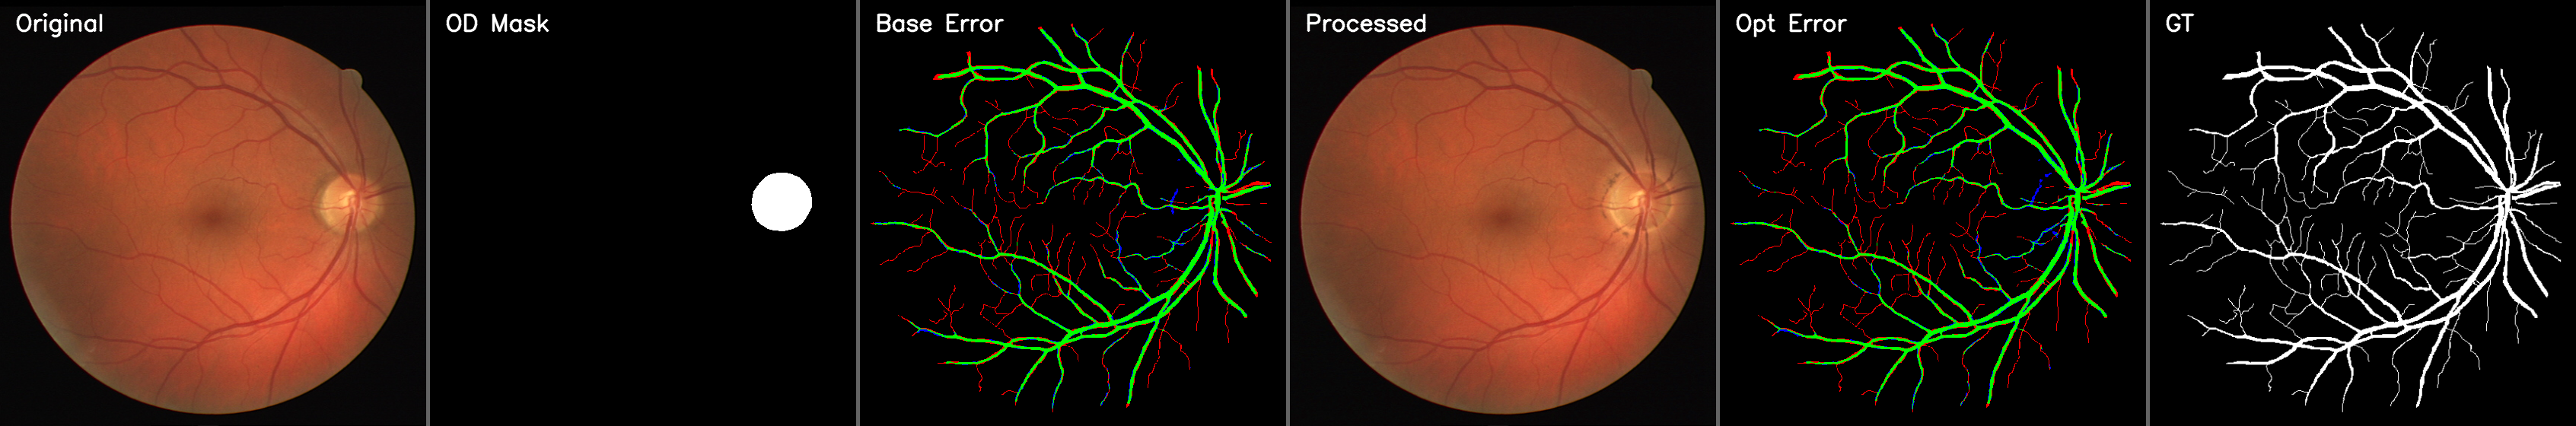
\includegraphics[width=0.9\linewidth]{figures/od_result_drive_10.png}
    \vspace{1pt}
    
    % --- 6. DRIVE 15 ---
    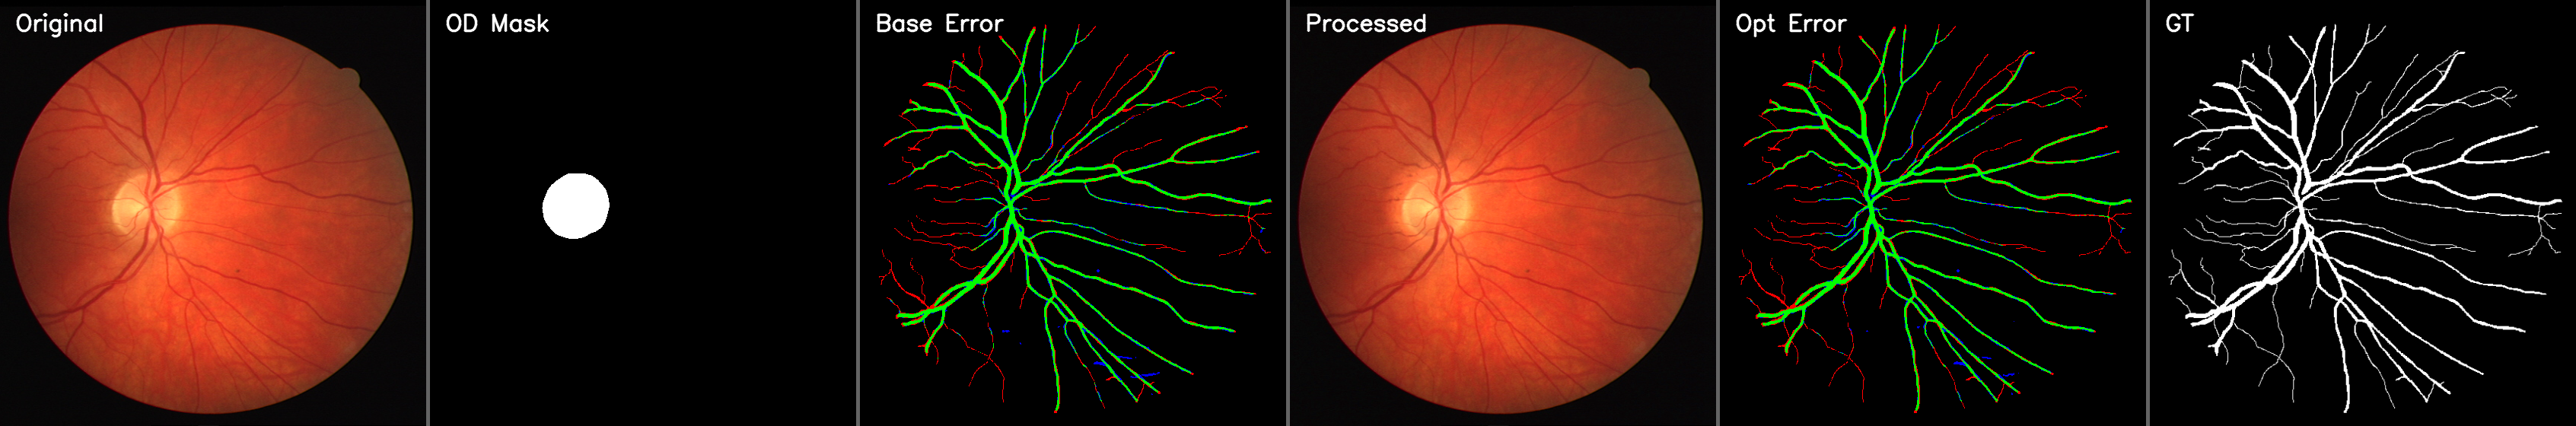
\includegraphics[width=0.9\linewidth]{figures/od_result_drive_15.png}
    \vspace{1pt}
    
    % --- 7. CHASE 01 ---
    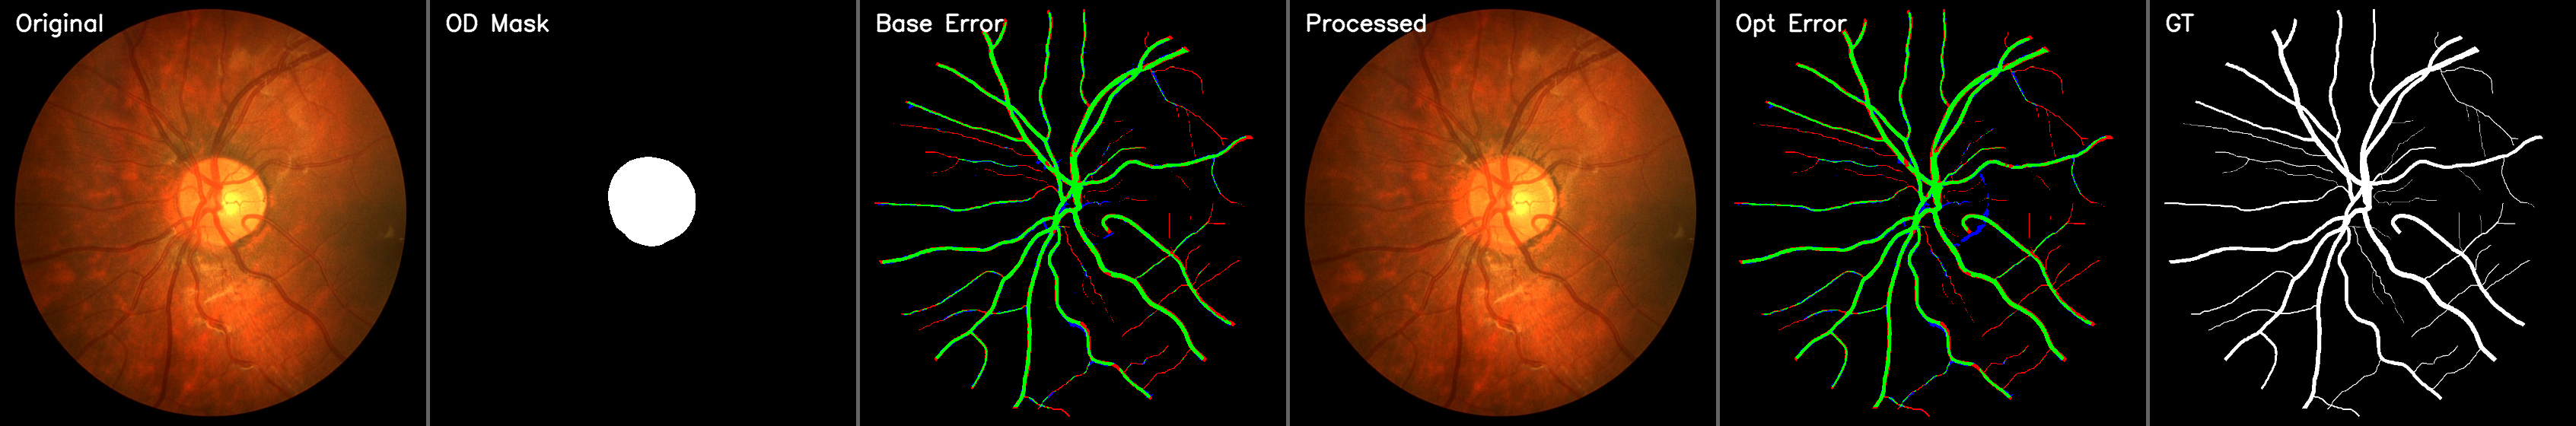
\includegraphics[width=0.9\linewidth]{figures/od_result_chase_01.png}
    \vspace{1pt}
    
    % --- 8. STARE 01 ---
    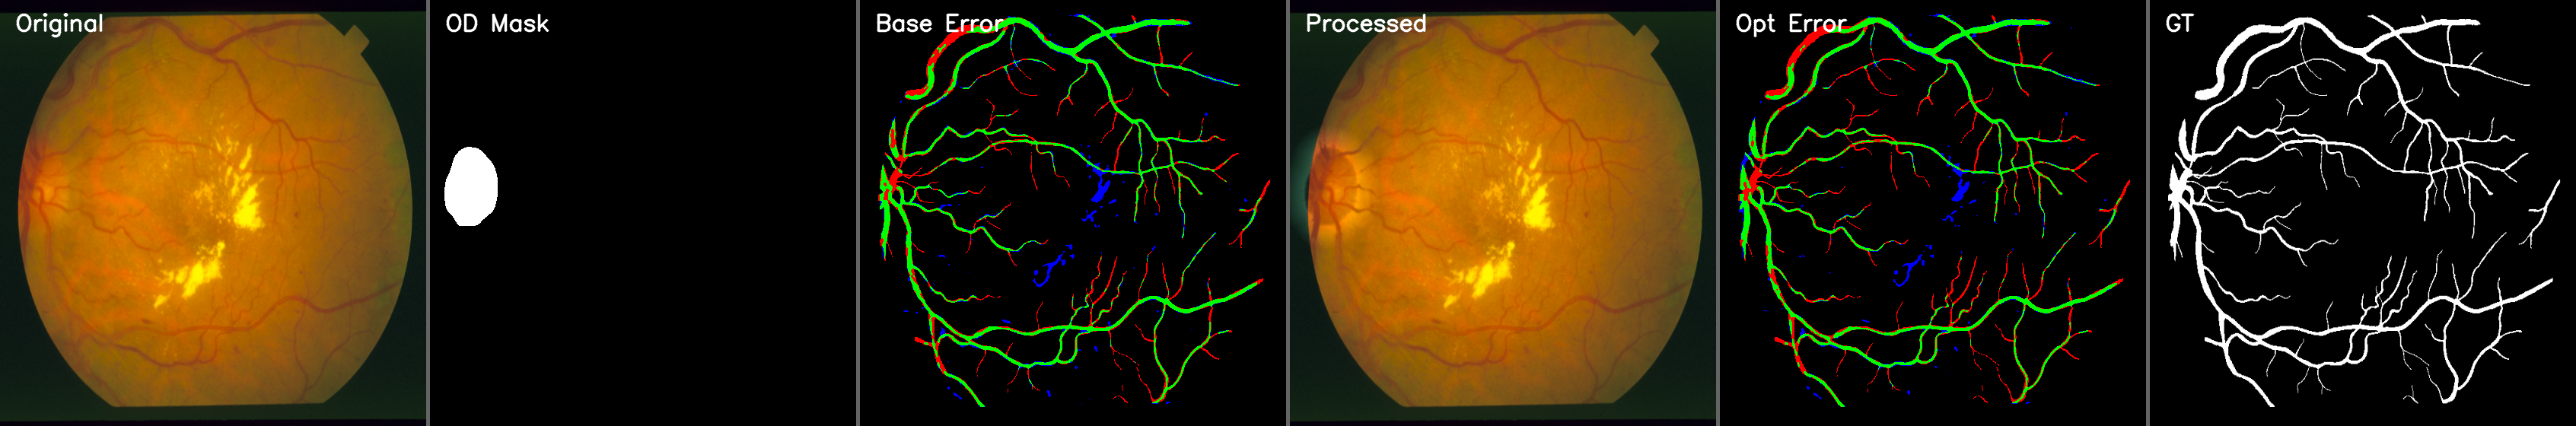
\includegraphics[width=0.9\linewidth]{figures/od_result_stare_01.png}

    % --- 总标题 ---
    \caption{视盘先验融合实验的可视化对比结果汇总。图片按从上到下的顺序排列，前5行展示了DRIVE数据集的不同样本（测试图 01, 02, 05, 10, 15），第7行为CHASE\_DB样本（01L），第8行为STARE样本（im0001）。每行图片内部从左到右依次为：(1)原始图像、(2)自动生成的视盘掩码、(3)基准模型误差图（绿=TP, 红=FN, 蓝=FP）、(4)处理后输入图像、(5)优化后模型误差图、(6)真值标注。}
    \label{fig:all_od_results}
\end{figure*}


\subsection{失败原因分析}

我们分析了导致失败的三个主要原因：

\subsubsection{语义冲突}
视盘区域同时包含：
\begin{itemize}
    \item 需要抑制的背景（视盘表面）
    \item 需要保留的主要血管（汇聚的动静脉）
\end{itemize}
二值视盘掩码无法区分这两种语义相反的区域，给网络造成混淆。

\subsubsection{误差传播}
自动生成的视盘掩码并非100\%准确。视盘掩码中的任何分割误差都会直接误导血管分割网络，导致系统性错误。

\subsubsection{特征稀释}
简单的输入通道拼接会导致空间先验信息在深层网络中逐渐衰减。当特征到达瓶颈层时，视盘位置信息已经被稀释。

\section{探索二：几何感知损失函数}

\subsection{动机}

鉴于显式视盘先验融合的失败，我们转向通过损失函数修改进行隐式几何建模。目标包括：
\begin{itemize}
    \item 解决血管与背景之间的类别不平衡问题
    \item 强制血管边缘的边界精度
    \item 减少视盘附近的假阳性
\end{itemize}

\subsection{方法}

\subsubsection{Focal Tversky损失}
我们使用Focal Tversky Loss\cite{salehi2017tversky}替换Dice损失，以控制FP/FN权衡：
\begin{equation}
    \mathcal{L}_{FT} = (1 - TI)^\gamma
\end{equation}
其中：
\begin{equation}
    TI = \frac{TP + \epsilon}{TP + \alpha \cdot FP + \beta \cdot FN + \epsilon}
\end{equation}
参数设置：$\alpha=0.7$，$\beta=0.3$，$\gamma=0.75$。

较高的$\alpha$值更严厉地惩罚假阳性，以解决视盘边界问题。

\subsubsection{边界损失}
使用Sobel边缘检测添加边界监督：
\begin{equation}
    \mathcal{L}_{Boundary} = \|G(\hat{Y}) - G(Y)\|_1
\end{equation}
其中$G(\cdot)$通过Sobel算子提取边界。

\subsubsection{组合损失}
\begin{equation}
    \mathcal{L}_{total} = \mathcal{L}_{FocalTversky} + 0.1 \cdot \mathcal{L}_{Boundary}
\end{equation}

\subsection{实验结果}

表\ref{tab:loss_results}展示了损失函数实验的结果。

\begin{table}[htbp]
\caption{DRIVE数据集上损失函数实验结果}
\label{tab:loss_results}
\centering
\begin{tabular}{@{}lccccc@{}}
\toprule
\textbf{方法} & \textbf{IoU} & \textbf{F1} & \textbf{敏感度} & \textbf{精确度} & \textbf{特异度} \\
\midrule
基准 & \textbf{0.631} & \textbf{0.773} & 0.698 & 0.873 & 0.990 \\
新损失 & 0.612 & 0.758 & 0.681 & \textbf{0.865} & \textbf{0.990} \\
+ DCN+SP & 0.608 & 0.755 & 0.680 & 0.858 & 0.989 \\
+ ASPP & 0.612 & 0.759 & 0.679 & 0.867 & 0.990 \\
\bottomrule
\end{tabular}
\end{table}

图\ref{fig:metrics_comparison}直观展示了不同方法在各项指标上的对比。

\begin{figure}[htbp]
\centering
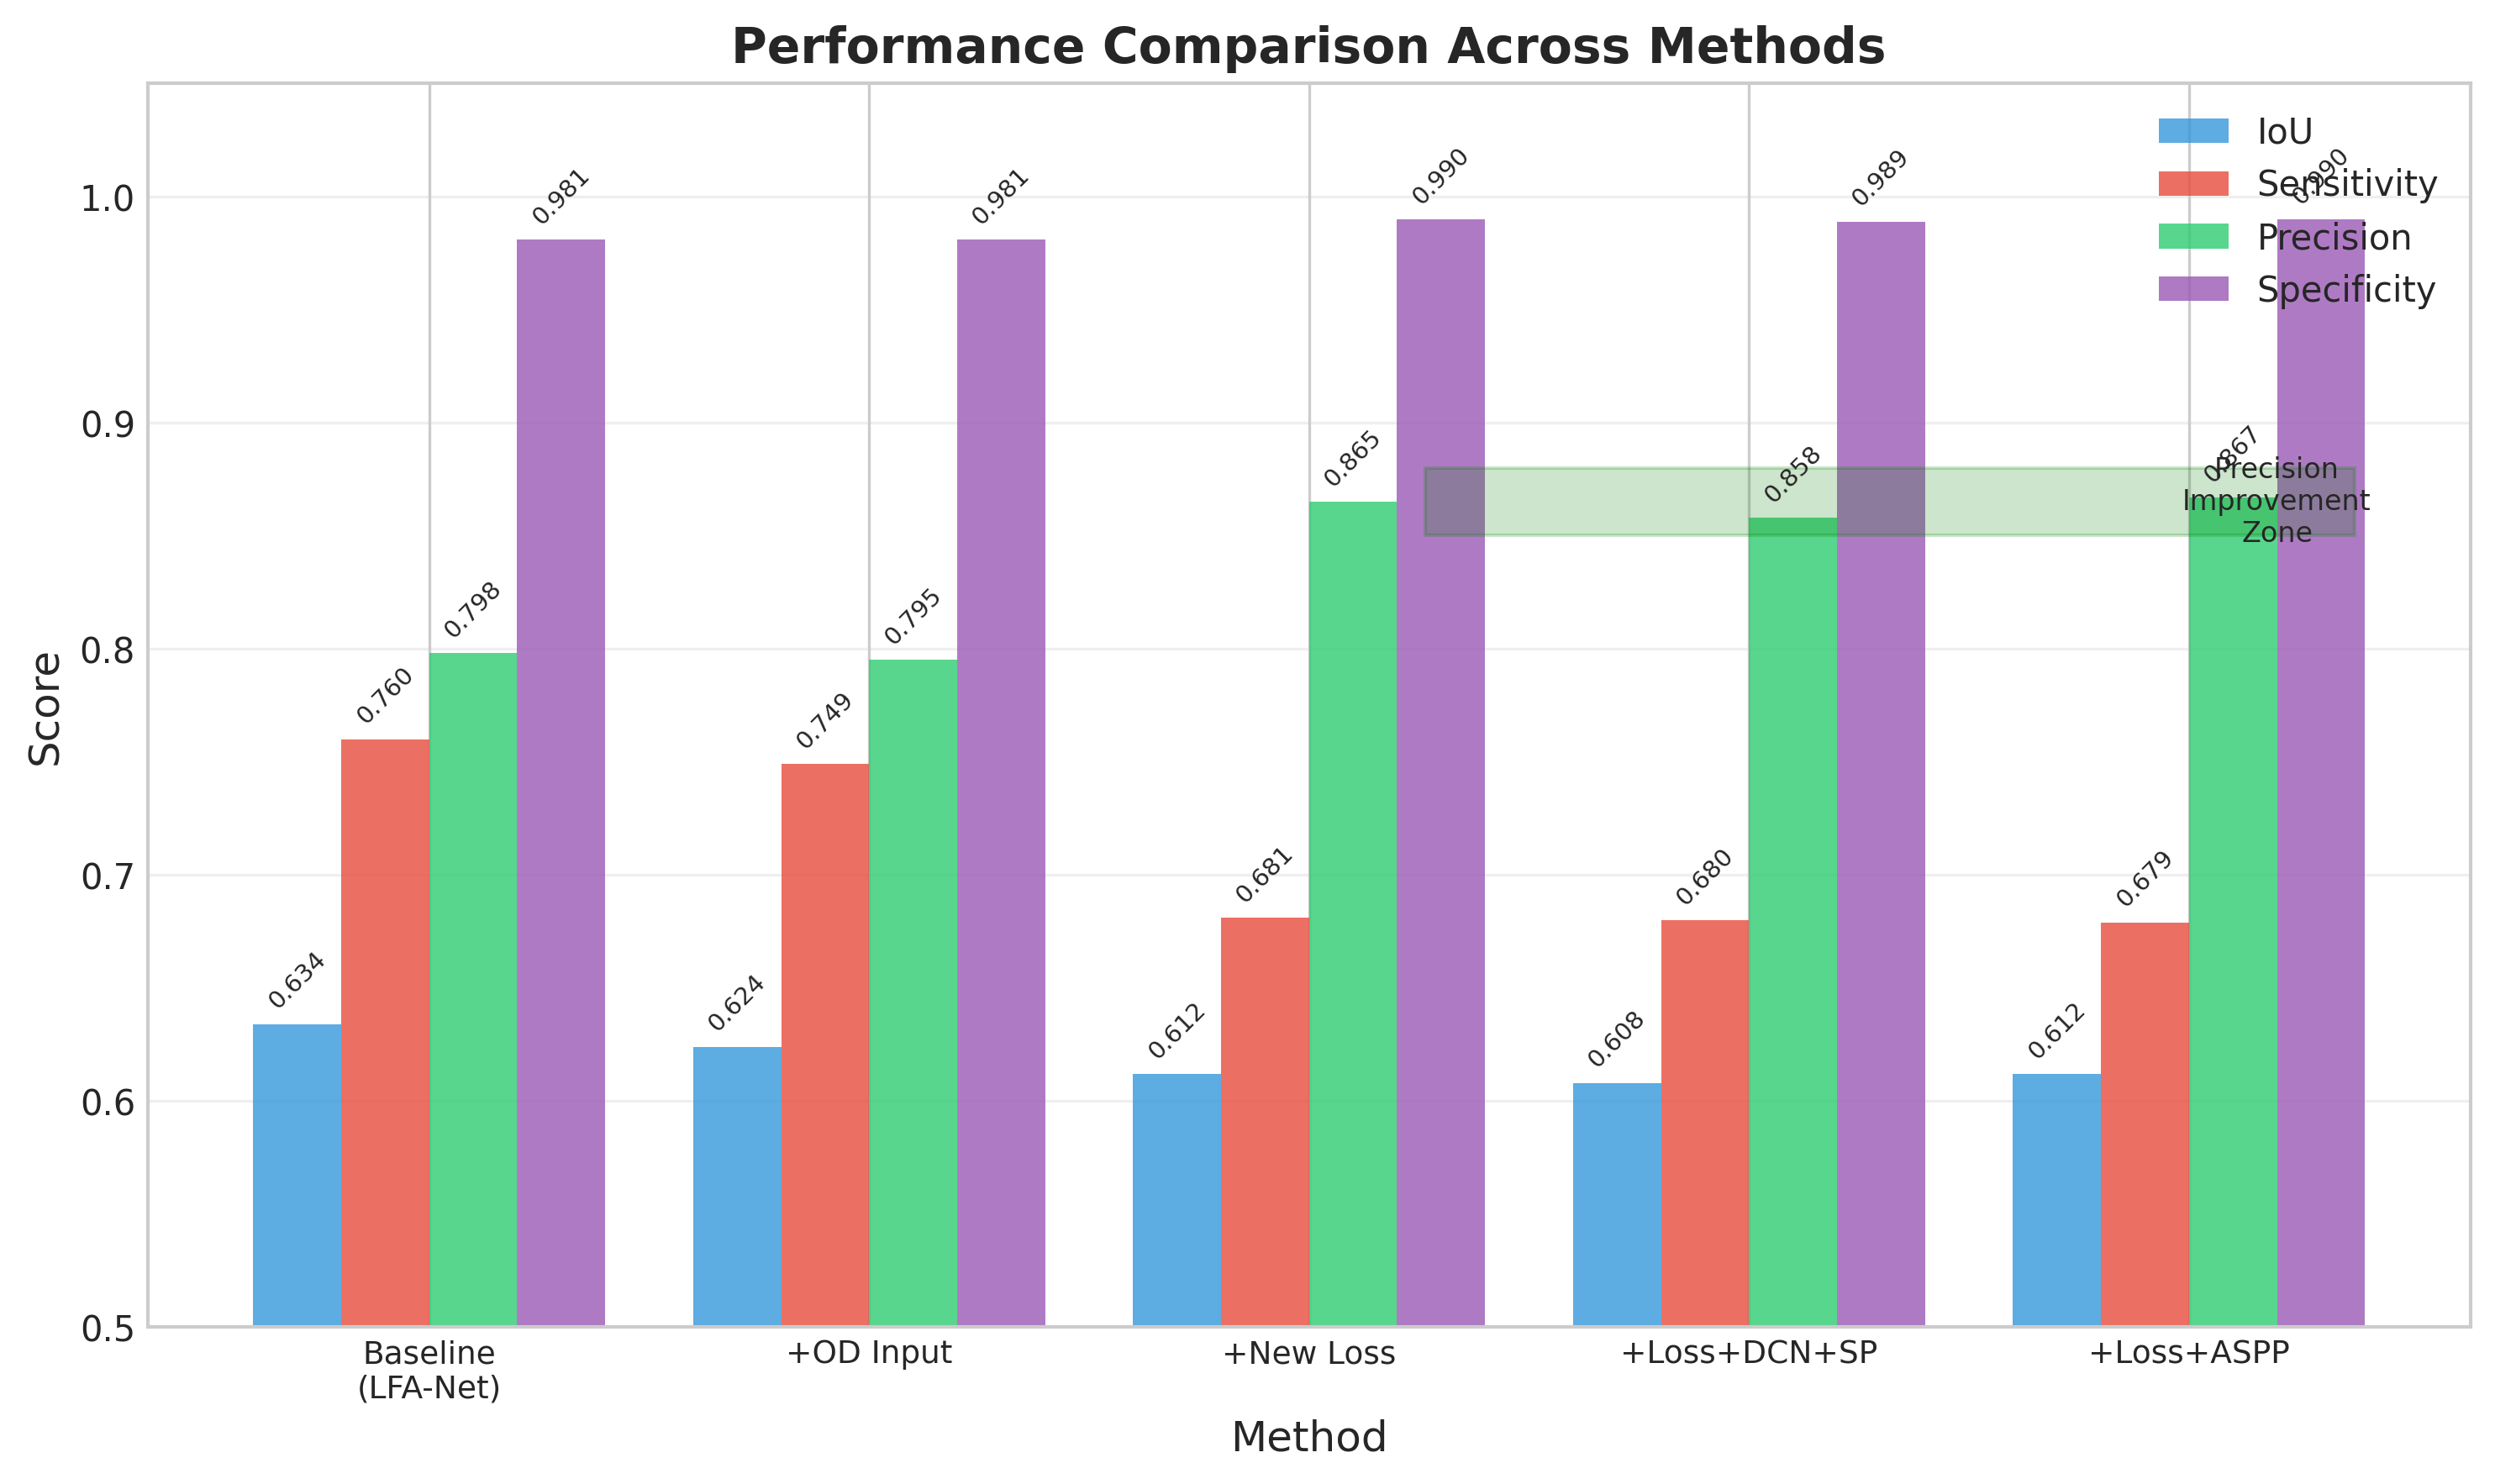
\includegraphics[width=0.95\columnwidth]{figures/metrics_comparison.png}
\caption{不同方法在DRIVE数据集上的性能指标对比。基准模型在IoU、F1和敏感度方面表现最优，而使用新损失函数的方法在精确度和特异度方面有明显提升。}
\label{fig:metrics_comparison}
\end{figure}

\subsection{结果分析}

结合表\ref{tab:baseline}（更新后的基准）与表\ref{tab:loss_results}（损失函数实验）的数据，我们需要对实验结果进行重新审视。与预期相反，引入复杂的几何感知损失函数并未带来性能提升，反而导致了指标的轻微回退。

\subsubsection{性能回退现象}
最新的基准测试表明，原版LFA-Net配合基础的DiceBCE损失已经达到了极高的性能水平（IoU 0.631, 精确度 0.873）。在此高基准下，Focal Tversky与边界损失的组合（新损失）表现如下：
\begin{itemize}
    \item \textbf{全面下降}：IoU从0.631降至0.612，F1从0.773降至0.758。
    \item \textbf{精确度未提升}：原本旨在抑制假阳性的高$\alpha$参数设置，并未能超越基准模型原本就已很高的精确度（0.873 $\rightarrow$ 0.865）。
    \item \textbf{敏感度损失}：模型对细微血管的捕捉能力进一步减弱（0.698 $\rightarrow$ 0.681）。
\end{itemize}

\subsubsection{失败原因深度剖析}
针对这一反直觉的结果，我们进行了深入分析，认为主要原因在于以下三点：

\paragraph{高基准效应与优化饱和}
基准LFA-Net模型虽然参数量极小（0.11M），但其设计中的LiteFusion模块已经极其高效地提取了特征。在DRIVE这样的小数据集（仅20张训练图）上，模型已经接近了性能饱和点。基础的DiceBCE损失提供了平滑且稳定的梯度，使得模型能够收敛到全局较优解。相比之下，引入额外的几何约束可能在优化平面上引入了不必要的局部极小值。

\paragraph{复杂损失的梯度噪声}
边界损失（Boundary Loss）依赖于距离变换图的回归，而Focal Tversky损失引入了非线性的指数调制。对于轻量级网络而言，这些复杂的损失函数在训练初期可能产生较大的梯度方差（Gradient Noise）。在没有预训练权重或更长训练周期的支持下，网络很难从这种复杂的损失地形中找到比DiceBCE更好的路径，导致最终收敛效果次优。

\paragraph{超参数的敏感性}
Focal Tversky损失中的$\alpha=0.7$是对假阳性的严厉惩罚。实验数据表明，基准模型的特异度已高达0.990，说明假阳性并非当前主要瓶颈。在这种情况下，过高的$\alpha$反而过度抑制了疑似血管像素的预测，导致模型变得“过于保守”，从而同时损害了精确度和敏感度。这提示我们在未来的工作中，应当采用可学习的或动态调整的损失权重，而非固定的超参数。


\section{额外架构实验}

我们还尝试了架构修改：

\subsection{ASPP模块}
在瓶颈层添加空洞空间金字塔池化\cite{chen2017deeplab}进行多尺度特征提取：
\begin{equation}
    \text{ASPP}(x) = \text{Conv}(\text{Concat}[f_1, f_6, f_{12}, f_{18}, \text{GAP}])
\end{equation}

\subsection{可变形卷积}
使用DCNv2\cite{dai2017deformable}替换标准卷积以适应弯曲的血管形状。可变形卷积通过学习采样位置偏移，能够更好地捕获不规则形状的结构。

\subsection{结果}
如表\ref{tab:loss_results}所示，当与新损失函数结合时，两种架构修改都未能改善结果。这表明：
\begin{itemize}
    \item 小规模训练集（20张图像）无法支撑额外的参数
    \item DCN的可学习偏移容易过拟合
    \item ASPP相比现有的多尺度ConvBlock收益有限
\end{itemize}

\section{讨论}

\subsection{经验教训}

\subsubsection{先验融合并非简单任务}
简单地将先验信息（视盘掩码）作为额外输入通道拼接是不够的。需要更复杂的融合机制：
\begin{itemize}
    \item 在跳跃连接处进行注意力门控融合
    \item 使用共享编码器的多任务学习
    \item 使用软注意力替代硬二值掩码
    \item 在解码器中引入条件归一化
\end{itemize}

\subsubsection{损失函数的权衡}
损失函数通过隐式优化目标控制模型行为。我们的实验表明：
\begin{itemize}
    \item 精确度和召回率往往相互对立
    \item 激进的假阳性抑制不可避免地损害敏感度
    \item 仔细的超参数调优至关重要
    \item 可能需要动态损失权重调度
\end{itemize}

\subsubsection{数据限制}
许多复杂技术需要比这些数据集提供的更多数据：
\begin{itemize}
    \item 20张训练图像限制了泛化能力
    \item 数据增强有帮助但无法完全弥补
    \item 跨数据集验证很重要
    \item 可考虑使用合成数据或迁移学习
\end{itemize}

\subsection{可能的改进方向}

基于我们的分析，潜在的改进包括：
\begin{enumerate}
    \item \textbf{动态损失权重}：从Dice开始，逐步引入边界损失
    \item \textbf{clDice损失}：基于骨架的拓扑保持\cite{shit2021cldice}
    \item \textbf{延长训练}：300轮以上配合学习率调度
    \item \textbf{基于注意力的视盘融合}：用注意力门控替代拼接
    \item \textbf{平衡的Tversky参数}：尝试$\alpha=0.3$，$\beta=0.7$以恢复敏感度
    \item \textbf{课程学习}：从简单样本开始，逐步增加难度
\end{enumerate}

\section{结论}

本项目在三个公开数据集（DRIVE、CHASE\_DB、STARE）上成功复现了LFA-Net基准模型。我们对视盘先验融合和几何感知损失函数的探索虽然未能提升定量指标，但提供了有价值的见解：

\begin{enumerate}
    \item LFA-Net是一个仅有0.11M参数的高效轻量级血管分割架构
    \item 通过输入拼接进行的简单先验融合由于语义冲突而无效
    \item 损失函数修改会产生需要仔细平衡的精确度-召回率权衡
    \item 小数据集显著限制了复杂技术的有效性
\end{enumerate}

损失函数实验中精确度和特异度的提升表明，该方法在假阳性率至关重要的临床筛查应用中可能具有价值。未来工作应探索动态损失调度和基于注意力的先验融合机制。


\begin{thebibliography}{00}

\bibitem{staal2004ridge}
J. Staal, M. D. Abràmoff, M. Niemeijer, M. A. Viergever, and B. van Ginneken, ``Ridge-based vessel segmentation in color images of the retina,'' \emph{IEEE Trans. Med. Imaging}, vol. 23, no. 4, pp. 501--509, 2004.

\bibitem{ronneberger2015u}
O. Ronneberger, P. Fischer, and T. Brox, ``U-Net: Convolutional networks for biomedical image segmentation,'' in \emph{Proc. MICCAI}, 2015, pp. 234--241.

\bibitem{lfanet2025}
LFA-Net Authors, ``LFA-Net: Lightweight network with litefusion attention for retinal vessel segmentation,'' \emph{arXiv preprint}, 2025.

\bibitem{oktay2018attention}
O. Oktay \emph{et al.}, ``Attention U-Net: Learning where to look for the pancreas,'' in \emph{Proc. MIDL}, 2018.

\bibitem{chen2017deeplab}
L.-C. Chen, G. Papandreou, I. Kokkinos, K. Murphy, and A. L. Yuille, ``DeepLab: Semantic image segmentation with deep convolutional nets, atrous convolution, and fully connected CRFs,'' \emph{IEEE TPAMI}, vol. 40, no. 4, pp. 834--848, 2018.

\bibitem{shit2021cldice}
S. Shit \emph{et al.}, ``clDice -- A novel topology-preserving loss function for tubular structure segmentation,'' in \emph{Proc. CVPR}, 2021.

\bibitem{xie2021segformer}
E. Xie, W. Wang, Z. Yu, A. Anandkumar, J. M. Alvarez, and P. Luo, ``SegFormer: Simple and efficient design for semantic segmentation with transformers,'' in \emph{Proc. NeurIPS}, 2021.

\bibitem{gu2019net}
Z. Gu \emph{et al.}, ``CE-Net: Context encoder network for 2D medical image segmentation,'' \emph{IEEE Trans. Med. Imaging}, vol. 38, no. 10, pp. 2281--2292, 2019.

\bibitem{li2018h}
L. Li, M. Verma, Y. Nakashima, H. Nagahara, and R. Kawasaki, ``IterNet: Retinal image segmentation utilizing structural redundancy in vessel networks,'' in \emph{Proc. WACV}, 2020.

\bibitem{guo2021sa}
C. Guo \emph{et al.}, ``SA-UNet: Spatial attention U-Net for retinal vessel segmentation,'' in \emph{Proc. ICPR}, 2020.

\bibitem{mou2019cs}
L. Mou \emph{et al.}, ``CS-Net: Channel and spatial attention network for curvilinear structure segmentation,'' in \emph{Proc. MICCAI}, 2019.

\bibitem{howard2017mobilenets}
A. G. Howard \emph{et al.}, ``MobileNets: Efficient convolutional neural networks for mobile vision applications,'' \emph{arXiv preprint arXiv:1704.04861}, 2017.

\bibitem{tan2019efficientnet}
M. Tan and Q. V. Le, ``EfficientNet: Rethinking model scaling for convolutional neural networks,'' in \emph{Proc. ICML}, 2019.

\bibitem{zhang2018shufflenet}
X. Zhang, X. Zhou, M. Lin, and J. Sun, ``ShuffleNet: An extremely computation-efficient CNN for mobile devices,'' in \emph{Proc. CVPR}, 2018.

\bibitem{kervadec2019boundary}
H. Kervadec, J. Bouchtiba, C. Desrosiers, E. Granger, J. Dolz, and I. Ben Ayed, ``Boundary loss for highly unbalanced segmentation,'' in \emph{Proc. MIDL}, 2019.

\bibitem{salehi2017tversky}
S. S. M. Salehi, D. Erdogmus, and A. Gholipour, ``Tversky loss function for image segmentation using 3D fully convolutional deep networks,'' in \emph{Proc. MLMI}, 2017.

\bibitem{lin2017focal}
T.-Y. Lin, P. Goyal, R. Girshick, K. He, and P. Dollár, ``Focal loss for dense object detection,'' in \emph{Proc. ICCV}, 2017.

\bibitem{aquino2010detecting}
A. Aquino, M. E. Gegúndez-Arias, and D. Marín, ``Detecting the optic disc boundary in digital fundus images using morphological, edge detection, and feature extraction techniques,'' \emph{IEEE Trans. Med. Imaging}, vol. 29, no. 11, pp. 1860--1869, 2010.

\bibitem{fu2018joint}
H. Fu \emph{et al.}, ``Joint optic disc and cup segmentation based on multi-label deep network and polar transformation,'' \emph{IEEE Trans. Med. Imaging}, vol. 37, no. 7, pp. 1597--1605, 2018.

\bibitem{fraz2012ensemble}
M. M. Fraz \emph{et al.}, ``An ensemble classification-based approach applied to retinal blood vessel segmentation,'' \emph{IEEE Trans. Biomed. Eng.}, vol. 59, no. 9, pp. 2538--2548, 2012.

\bibitem{hoover2000locating}
A. Hoover, V. Kouznetsova, and M. Goldbaum, ``Locating blood vessels in retinal images by piecewise threshold probing of a matched filter response,'' \emph{IEEE Trans. Med. Imaging}, vol. 19, no. 3, pp. 203--210, 2000.

\bibitem{dai2017deformable}
J. Dai \emph{et al.}, ``Deformable convolutional networks,'' in \emph{Proc. ICCV}, 2017.

\end{thebibliography}

\end{CJK}
\end{document}
